\begin{frame}{Լրիվ գրաֆների միջակայքային ներկումներ}{$W(K_{2n})$ պարամետրի ստորին գնահատականներ}



\begin{itemize}
\item Եթե $n\in \mathbb{N}$, ապա $W(K_{2n}) \geq 3n-2$ (Պետրոսյան, 2010)
\end{itemize}

\begin{theorem}[1.4.2]
Եթե $n \geq 2$, ապա $W(K_{2n}) \geq \lfloor 3.5n \rfloor - 3$:
\end{theorem}

\begin{figure}[b!]
\centering
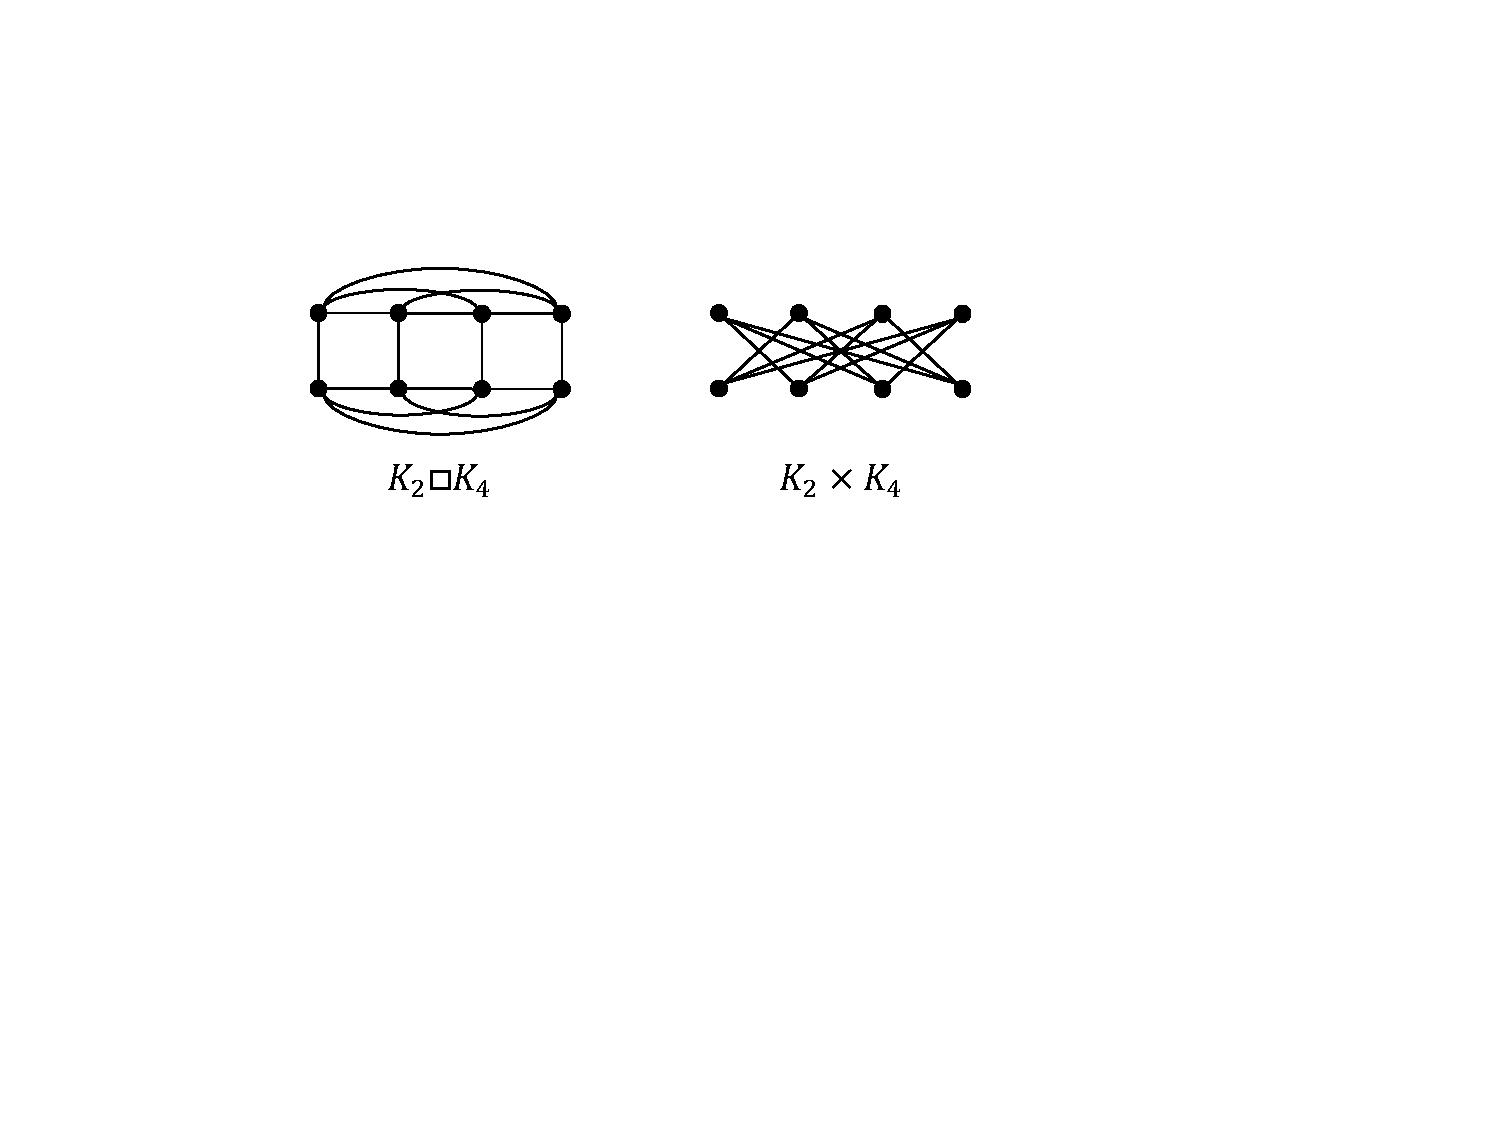
\includegraphics[width=0.8\textwidth]{figures/K_8products.pdf}
\label{K_8products}
\end{figure}

\end{frame}

\begin{frame}{Լրիվ գրաֆների միջակայքային ներկումներ}{$W(K_{2n})$ պարամետրի ստորին գնահատականներ}

\begin{itemize}
\item Ցանկացած $n\in \mathbb{N}$ թվի համար $W(K_{4n}) \geq W(K_{2n}) + 4n-1$ (Պետրոսյան, 2010)
\end{itemize}

\begin{theorem}[1.4.4]
Ցանկացած $m,n \in\mathbb{N}$ թվերի համար
\begin{center}
$W(K_{2mn}) \geq W(K_{2m}) + W(K_{2n}) + 4(m-1)(n-1) - 1$:
\end{center}
\end{theorem}

\begin{figure}[t!]
\centering
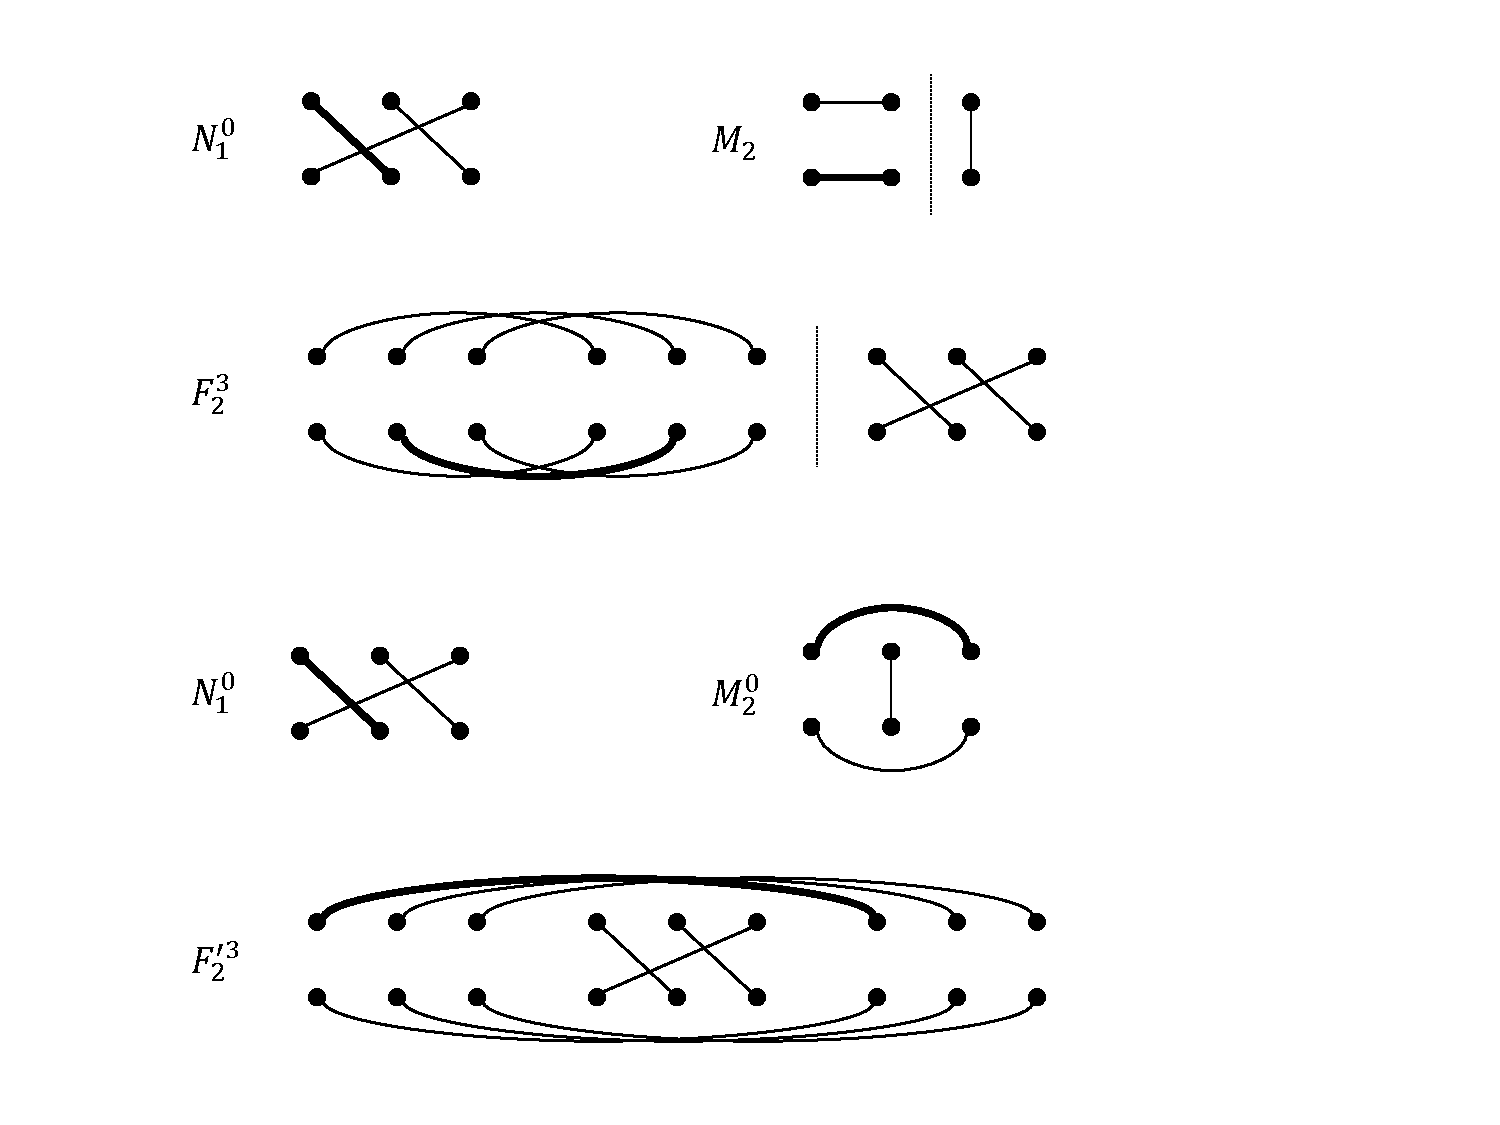
\includegraphics[trim={0 10cm 0 0cm},clip,width=0.4\textwidth]{figures/K_18-2.pdf}
\hspace{0.5cm}
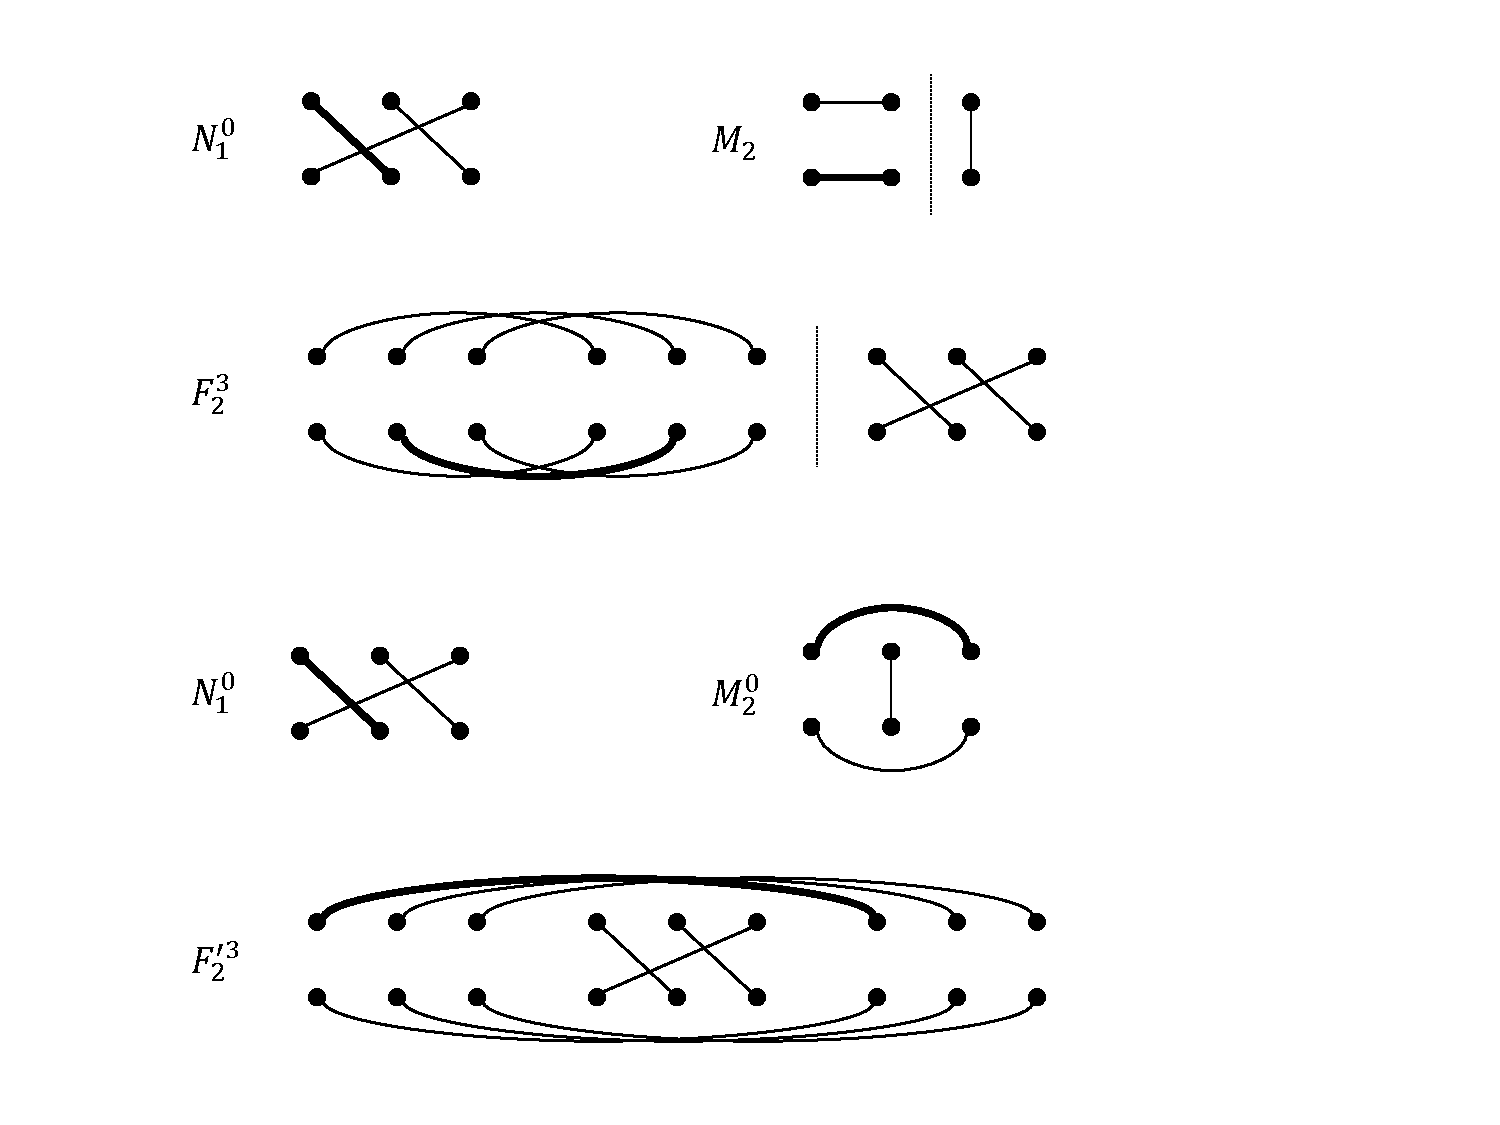
\includegraphics[trim={0 0.4cm 0 9cm},clip,width=0.4\textwidth]{figures/K_18-2.pdf}
\end{figure}

% Քանի որ $W(K_6) = 7$ և $W(K_{10}) \geq 14$, ուստի $W(K_{30}) \geq 52$, հետևաբար այս արդյունքը հերքում է Հիպոթեզ \ref{h1_complete_log}-ը, ըստ որի $W(K_{30})=51$: 

\end{frame}

\begin{frame}{Լրիվ գրաֆների միջակայքային ներկումներ}{$W(K_{2n})$ պարամետրի ստորին գնահատականներ}

\begin{theorem}[1.4.5]
Եթե $n = \prod\limits_{i=1}^{\pi(n)}{p_i^{\alpha_i}}$, որտեղ $p_i$-ն $i$-րդ պարզ թիվն է, $\pi(n)$-ը՝ $n$-ը չգերազանցող պարզ թվերի քանակը, իսկ $\alpha_i \in \mathbb{Z}_{\geq 0}$, ապա
\begin{center}
$W(K_{2n}) \geq 4n - 3 - \sum\limits_{i=1}^{\pi(n)}{\alpha_i\left(4p_i-3-W(K_{2p_i})\right)}$:
\end{center}
\end{theorem}

\end{frame}

\begin{frame}{Լրիվ գրաֆների միջակայքային ներկումներ}{$W(K_{2n})$ պարամետրի վերին գնահատական}

\begin{itemize}
\item Եթե $n \geq 2$, ապա 
\begin{center}
$W(K_{2n}) \leq 4n-4$
\end{center} (Գիառո, Կուբալ, Մալաֆիյսկի, 2001)
\end{itemize}

\begin{theorem}[1.4.17]
Եթե $n \geq 3$, ապա
\begin{center}
$W(K_{2n}) \leq \left\{
\begin{tabular}{ll}
$4n-5$, & երբ $n \geq 3$,\\
$4n-6$, & երբ $n \geq 5$,\\
$4n-7$, & երբ $n \geq 9$:\\
\end{tabular}
\right.$
\end{center}
\end{theorem}

% 1.4 պարագրաֆի վերջում որոշվել են նաև $W(K_{2n})$ պարամետրի ճշգրիտ արժեքները, երբ $n \leq 12$ և $n=16$ (Աղյուսակ \ref{tableAll}): Այս արդյունքների համադրմամբ ստացվել է հետևյալ ստորին գնահատականը.
\end{frame}

\begin{frame}{Լրիվ գրաֆների միջակայքային ներկումներ}{$W(K_{2n})$ պարամետրի ստորին գնահատականներ}

Եթե $n=p2^{q}$, որտեղ $p$-ն կենտ է, իսկ $q \in \mathbb{Z}_{\geq 0}$, ապա
\begin{center}
$W\left(K_{2n}\right)\geq 4n-2-p-q$
\end{center} 
(Պետրոսյան, 2010)

\begin{theorem}[1.4.20]
Եթե $n = \prod\limits_{i=1}^{\pi(n)}{p_i^{\alpha_i}}$, որտեղ $p_i$-ն $i$-րդ պարզ թիվն է, $\pi(n)$-ը՝ $n$-ը չգերազանցող պարզ թվերի քանակը, իսկ $\alpha_i \in \mathbb{Z}_{\geq 0}$, ապա 
\begin{center}
$W(K_{2n}) \geq 4n - 3 - A_n$,
\end{center}
որտեղ $A_n = \alpha_1 + 2\alpha_2 + 3\alpha_3 + 4\alpha_4 + 4\alpha_5 + \frac{1}{2}\sum\limits_{i=6}^{\pi(n)}{\alpha_i(p_i+1)}$:
\end{theorem}

\end{frame}


\begin{frame}{Լրիվ գրաֆների միջակայքային ներկումներ}{$W(K_{2n})$ պարամետրի ճշգրիտ արժեքներ}
Ճշգրիտ արժեքները հայտնի են, երբ $n \leq 12$ և $n=16$:

\fontsize{7pt}{14}\selectfont
\begin{table}[h]
\centering
\begin{tabularx}{0.96\textwidth}{r||*{18}{c<{\hspace{-4.5pt}}|}}
$n$ 
& $1$ & $2$ & $3$ & $4$ & $5$ & $6$ & $7$ & $8$ & $9$ & $10$ & $11$ & $12$ & $13$ & $14$ & $15$ & $16$  \\ \hline\hline
$W(K_{2n}) \geq $ 
& $1$ & $4$ & $7$ & $11$ & $14$ & $18$ & $21$ & $26$ & $29$ & $33$ & $37$ & $41$ & $42$ & $46$ & $52$ & $57$ \\ \hline
$W(K_{2n}) = $
& $1$ & $4$ & $7$ & $11$ & $14$ & $18$ & $21$ & $26$ & $29$ & $33$ & $37$ & $41$ &  &  &  & $57$  \\ \hline
$W(K_{2n}) \leq $
& $1$ & $4$ & $7$ & $11$ & $14$ & $18$ & $22$ & $26$ & $29$ & $33$ & $37$ & $41$ & $45$ & $49$ & $53$ & $57$ 
\end{tabularx}
\end{table}
% \pause

% \fontsize{11pt}{12}\selectfont
% 2016-ին Հուդակը, Կարդոշը, Մադարասը և Վրբյարովան դիտարկել են այս խնդիրը առանց ներկման ճշտության պայմանի: \\Նրանք ցույց են տվել, որ այդ դեպքում գագաթների թվից կախված գույների քանակը խիստ աճում է:
\end{frame}